\chapter{Implementacija i korisničko sučelje}
		
		
		\section{Korištene tehnologije i alati}
		
%			\textbf{\textit{dio 2. revizije}}
%			
%			 \textit{Detaljno navesti sve tehnologije i alate koji su primijenjeni pri izradi dokumentacije i aplikacije. Ukratko ih opisati, te navesti njihovo značenje i mjesto primjene. Za svaki navedeni alat i tehnologiju je potrebno \textbf{navesti internet poveznicu} gdje se mogu preuzeti ili više saznati o njima}.


			\begin{enumerate}
				\item \textbf{Java}\\
				- Objektno orijentirani programski jezik koji smo koristili za izradu naše backend aplikacije.\\
				- \url{https://docs.oracle.com/en/java/}
				
				\item \textbf{Spring Boot}\\
				- Radni okvir(engl. \textit{framework}) koji smo koristili za efikasniju izradu backend aplikacije koju smo pisali u programskom jeziku Java. Sadrži velik niz već uključenih knjižnica, kao što su Jackson, Hibernate itd.\\
				- \url{https://spring.io/projects/spring-boot}
				
				\item \textbf{Hibernate ORM}\\
				- Alat koji omogućava pretvorbu tj. mapiranje redova iz tablice baze podataka u objekte Java aplikacije.\\
				- \url{https://hibernate.org/orm/}
				
				\item \textbf{Jackson}\\
				- Knjižnica(engl. \textit{library}) koja omogućava pretvorbe između objekata u Java aplikaciji i Stringova u JSON formatu.\\
				- \url{https://github.com/FasterXML/jackson-docs}
				
				\item \textbf{React}\\
				- Knjižnica koju smo koristili za efikasniju izradu frontend aplikacije tj. korisničkog sučelja za čiju izradu su se koristile tri glavne web tehnologije (HTML, CSS, Javascript).\\
				- \url{https://reactjs.org/}
				
				\item \textbf{HTML}\\
				- Osnovni jezik za izradu web stranica. Stvara html elemente, ali ne podržava veću stilizaciju tih elemenata.\\
				- \url{https://developer.mozilla.org/en-US/docs/Web/HTML}
				
				\item \textbf{CSS} \\
				- Jezik za uređivanje html elemenata tj. stiliziranje web stranice. \\
				- \url{https://developer.mozilla.org/en-US/docs/Web/CSS}
				
				\item \textbf{Javascript} \\
				- Programski jezik koji smo koristili za implementaciju funkcionalnosti na frontend aplikaciji.\\
				- \url{https://developer.mozilla.org/en-US/docs/Web/JavaScript}
				
				\item \textbf{React Bootstrap}\\
				- Radni okvir koji sadrži veliku količinu već uređenih React komponenti.\\
				- \url{https://react-bootstrap.github.io/}
				
				\item \textbf{Git}\\
				- Distribuirani sustav za upravljanje različitim verzijama podataka (npr. programskog koda ili teksta).\\
				- \url{https://git-scm.com/}
				
				\item \textbf{Gitlab}\\
				- Web platforma na kojoj se nalazi naš udaljeni git repozitorij.\\
				- \url{https://about.gitlab.com/}
				
				\item \textbf{Slack}\\
				- Platforma koju smo koristili za komunikaciju unutar tima.\\
				- \url{https://slack.com/intl/en-hr/}
				
				\item \textbf{Heroku}\\
				- Platforma na kojoj se poslužuje naša web aplikacija (frontend, backend i baza podataka).\\
				- \url{https://www.heroku.com/home}
				
				\item \textbf{PostgreSQL}\\
				- Sustav za upravljanje bazom podataka koji smo koristili za relacijsku bazu podataka za našu aplikaciju.\\
				- \url{https://www.postgresql.org/}
				
				\item \textbf{Intellij IDEA}\\
				- Integrirana razvojna okolina koja služi primarno za pisanje Java aplikacija, ali ju je osim backend tima, koristio i frontend tim.\\
				- \url{https://www.jetbrains.com/idea/}
				
				\item \textbf{Eclipse} \\
				- Integrirana razvojna okolina za pisanje Java aplikacija koju je koristio dio backend tima.\\
				- \url{https://www.eclipse.org/}
				
				\item \textbf{Visual Studio Code}\\
				- Razvojna okolina koja podržava mnoge tehnologije, a u našem timu ju je koristio frontend tim.\\
				- \url{https://code.visualstudio.com/}
				
				\item \textbf{PgAdmin4}\\
				- Alat za upravljanje PostgreSQL bazom podataka.\\
				- \url{https://www.pgadmin.org/}
				
				\item \textbf{Swagger2}\\
				- Alat koji smo koristili za lakšu komunikaciju backenda i frontenda. Alat iz programskog koda dokumentira cijeli API, te podržava grafičko sučelje koje je frontend tim koristio kako bi se informirao o API-ju kojeg treba koristiti.\\
				- \url{https://swagger.io/}
				
				\item \textbf{HERE REST APIs}\\
				- Besplatni API koji smo koristili za geokodiranje adresa iz naše aplikacije.\\
				- \url{https://developer.here.com/develop/rest-apis}
				
			\end{enumerate}
		 
			
			\eject 
		
	
		\section{Ispitivanje programskog rješenja}
			
%			\textbf{\textit{dio 2. revizije}}\\
%			
%			 \textit{U ovom poglavlju je potrebno opisati provedbu ispitivanja implementiranih funkcionalnosti na razini komponenti i na razini cijelog sustava s prikazom odabranih ispitnih slučajeva. Studenti trebaju ispitati temeljnu funkcionalnost i rubne uvjete.}
%	
			
			\subsection{Ispitivanje komponenti}
			Pomoću JUnit 4 napravljeno je 12 testova za klasu UsersService kojima se testiraju CRUD operacije spremanja,brisanja i dohvaćanja korisnika.
			\begin{lstlisting}
		
			@SpringBootTest
			public class UpravljanjeKucnimOtpadomApplicationTests {
				@Autowired
				private UsersService serv;
				
				@Test
				public void returnsEmptyIfUserIsNotFOund() {
					assertEquals(Optional.empty(), serv.getUser(-1));
				}
				
				@Test(expected=BadRequestException.class)
				public void cantCreateTwoUsersWithSameUsername() {
					serv.saveUser("Username", "password", "firstName", "lastName", "city", "street",1, "email10", Role.ADMIN);//dodan
					serv.saveUser("Username", "password", "firstName", "lastName", "city", "street",1, "email9", Role.ADMIN);
					fail();
				}
				
				@Test(expected=IllegalArgumentException.class)
				public void userNameCantBeNull() {
					serv.saveUser(null, "password", "firstName", "lastName", "city", "street",1, "email8", Role.ADMIN);
					fail();
				}
				
				@Test(expected=IllegalArgumentException.class)
				public void userNameCantBeBlank() {
					serv.saveUser("", "password", "firstName", "lastName", "city", "street",1, "email6", Role.ADMIN);
					fail();
				}
				
				@Test(expected=IllegalArgumentException.class)
				public void passwordNameCantBeNull() {
					serv.saveUser("Username", null, "firstName", "lastName", "city", "street",1, "email7", Role.ADMIN);
					fail();
				}
				
				@Test(expected=IllegalArgumentException.class)
				public void passwordNameCantBeBlank() {
					serv.saveUser("Username", "", "firstName", "lastName", "city", "street",1, "email5", Role.ADMIN);
					fail();
				}
				
				@Test(expected=IllegalArgumentException.class)
				public void passwordLengthMustBeGreaterOrEquals8() {
					serv.saveUser("Username", "passwor", "firstName", "lastName", "city", "street",1, "email4", Role.ADMIN);
					fail();
				}
				
				@Test(expected=IllegalArgumentException.class)
				public void roleMustNotBeNull() {
					serv.saveUser("Username", "password", "firstName", "lastName", "city", "street",1, "email3", null);
					fail();
				}
				
				@Test
				public void getByUsername() {
					serv.saveUser("Usernamee", "password", "firstName", "lastName", "city", "street",1, "email", Role.ADMIN);//dodan
					User user=serv.getUserByUsername("Usernamee").get();
					if(!user.getUsername().equals("Usernamee")) {
						fail();
					}
				}
				
				@Test
				public void userDeleteTest() {
					serv.saveUser("Username", "password", "firstName", "lastName", "city", "street",1, "email1", Role.ADMIN);//dpdam
					User toBeDeleted=serv.getUserByUsername("Username").get();
					serv.deleteUser(toBeDeleted.getID());
				}
				
				@Test(expected=BadRequestException.class)
				public void createTwoUsersWithSameEmails() {
					serv.saveUser("Username", "password", "firstName", "lastName", "city", "street",1, "emailsame", Role.ADMIN);//dodan
					serv.saveUser("User", "password", "firstName", "lastName", "city", "street",1, "emailsame", Role.ADMIN);
					fail();
				}
				
				@Test
				public void getAllUsers() {
					serv.saveUser("User", "password", "firstName", "lastName", "city", "street",1, "emailsame", Role.ADMIN);//dodan
					serv.saveUser("Username", "password", "firstName", "lastName", "city", "street",1, "email1", Role.ADMIN);//dodam
					serv.saveUser("Userr", "password", "firstName", "lastName", "city", "street",1, "email10", Role.ADMIN);//dodan
					if(serv.getUsers().size()!=3){
						System.out.println(serv.getUsers().size());
						fail();
					}
				}
			}
			\end{lstlisting}
			\begin{figure}[H]
				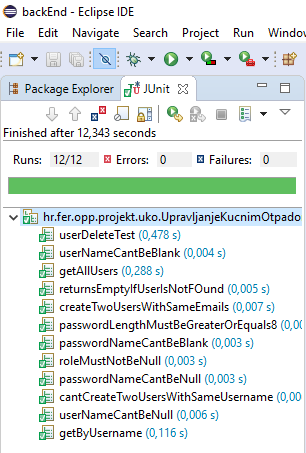
\includegraphics{slike/JUnit 4 testovi.png}
				\centering
				\caption{JUnit 4 testovi}
				\label{fig:JUnit 4 testovi}
			\end{figure}

			
			
			\subsection{Ispitivanje sustava}
			
			Ispitivanje sustava se izvodilo pomoću dodatka za preglednik Selenium IDE. U nastavku će se pokazati primjeri ispitivanja rubnih slučajeva, pozivanje funkcionalnosti koja nije potpuno implementirana te ispitivanje redovitih slučajeva.\\\\
			
			\textbf{Ispitni slučaj 1: Registracija korisnika s postojećim usernameom}
			\text{}\\
			
			\textbf{Ulaz:}
			
			\begin{packed_enum}
				\item{Otvaranje stranice za registraciju u web pregledniku}
				\item{Upisivanje podataka za korisnika s već postojećim username podatkom}
			\end{packed_enum}
		
			\textbf{Očekivani rezultat:}
			
			\begin{packed_enum}
				\item{Pojavljivanje upozorenja da username već postoji}
				\item{Registracija ne prolazi}
			\end{packed_enum}
		
			\textbf{Rezultat:} Pojavilo se upozorenje. Aplikacija je prošla test
			
		
			\begin{figure}[H]
				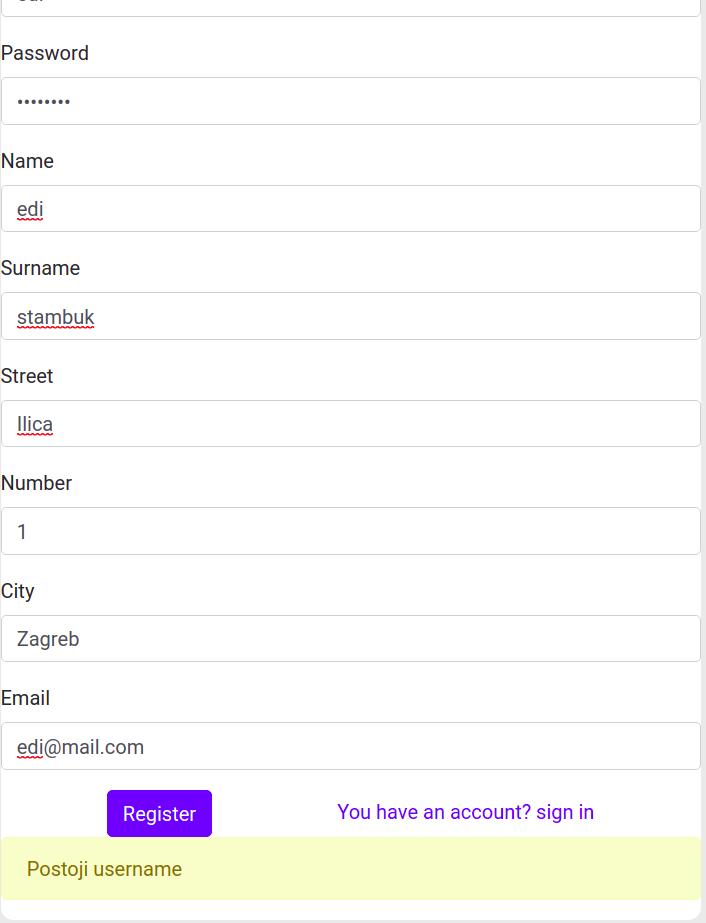
\includegraphics[scale=0.4]{slike/Upozorenje.png}
				\centering
				\caption{Upozorenje}
				\label{fig:Upozorenje}
			\end{figure}
			
			\text{}\\
		
		
			\textbf{Ispitni slučaj 2: Upisivanje slova u polje za upis vremena}
			\text{}\\
			
			\textbf{Ulaz:}
			
			\begin{packed_enum}
				\item{prijavljivanje kao zaposlenik ili administrator}
				\item{Otvaranje stranice za dostupnost odlagališta}
				\item{Pritisak mišem na lokaciju na karti}
				\item{Ažuriranje podataka za lokaciju}
				\item{upisivanje slova u polje za upis vremena}
			\end{packed_enum}
			
			\textbf{Očekivani rezultat:}
			
			\begin{packed_enum}
				\item{Pojavljivanje greške zbog netočnog formata datuma}
			\end{packed_enum}
			
			\textbf{Rezultat:} Korisnik se nije registrirao i nije se pojavila greška zbog netočnog upisa. Aplikacija nije prošla test
			
			\begin{figure}[H]
				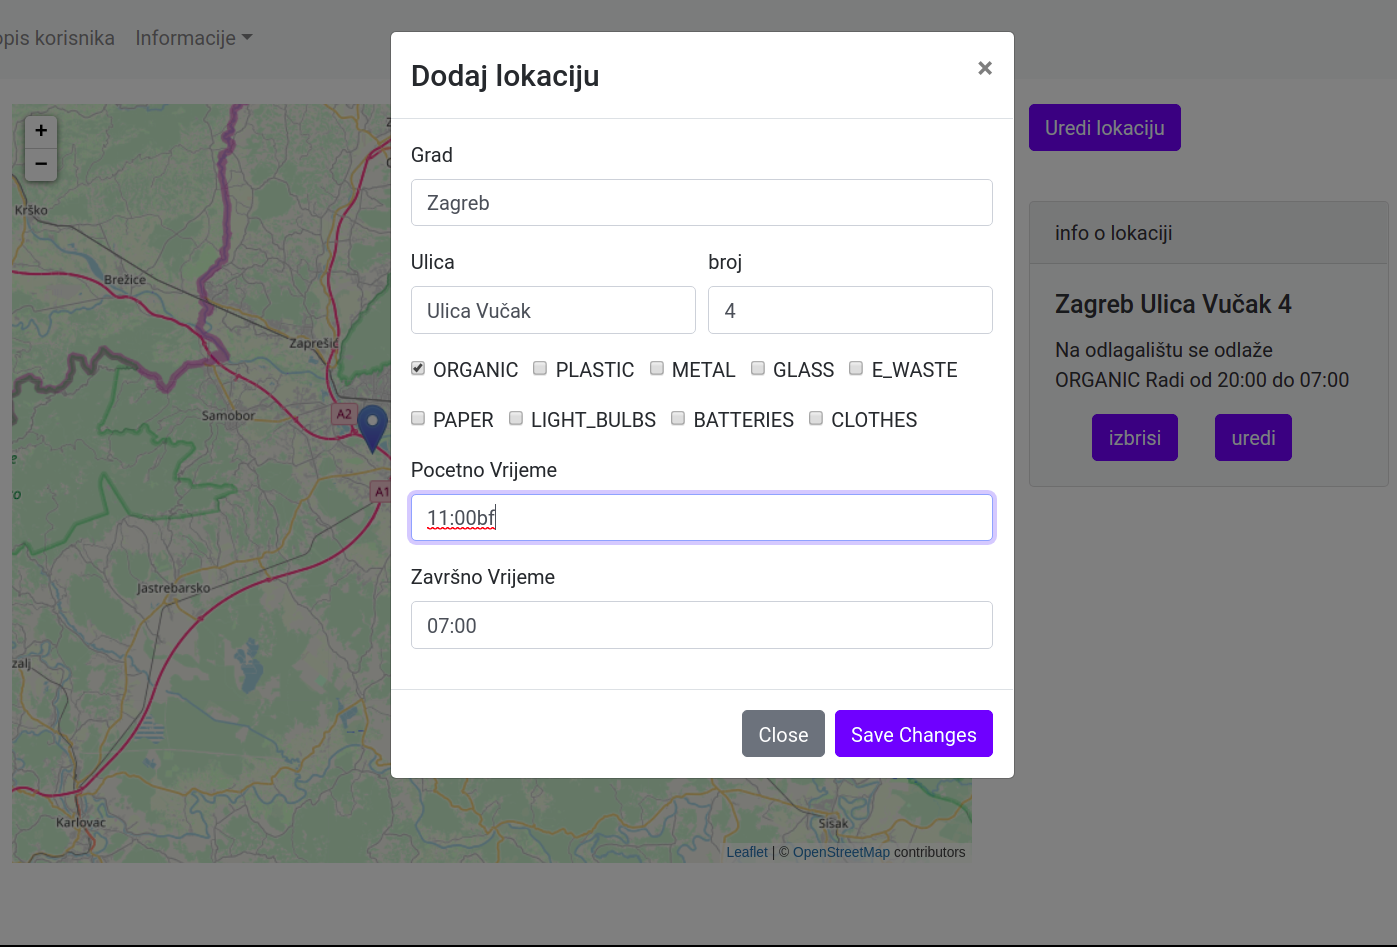
\includegraphics[scale=0.3]{slike/Netocan_upis.png}
				\centering
				\caption{Upis slova u komponentu za vrijeme}
				\label{fig:Netocan_upis}
			\end{figure}
		
			\text{}\\\\
		
			\textbf{Ispitni slučaj 3: Uspješno slanje zahtjeva za resursima}
			\text{}\\
			
			\textbf{Ulaz:}
			
			\begin{packed_enum}
				\item{Prijavljivanje kao građanin}
				\item{Otvaranje stranice za slanje zahtjeva za resursima}
				\item{Odabir resursa i broj traženih resursa}
				\item{Pritisak na gumb pošalji}
			\end{packed_enum}
			
			\textbf{Očekivani rezultat:}
			
			\begin{packed_enum}
				\item{Pojavljivanje informacija o poslanom zahtjevu}
				\item{Pojavljivanje zahtjeva na listi poslanih zahtjeva}
			\end{packed_enum}
			
			\textbf{Rezultat:} Korisnik je uspješno poslao zahtjev. Aplikacija je prošla test
			
			\begin{figure}[H]
				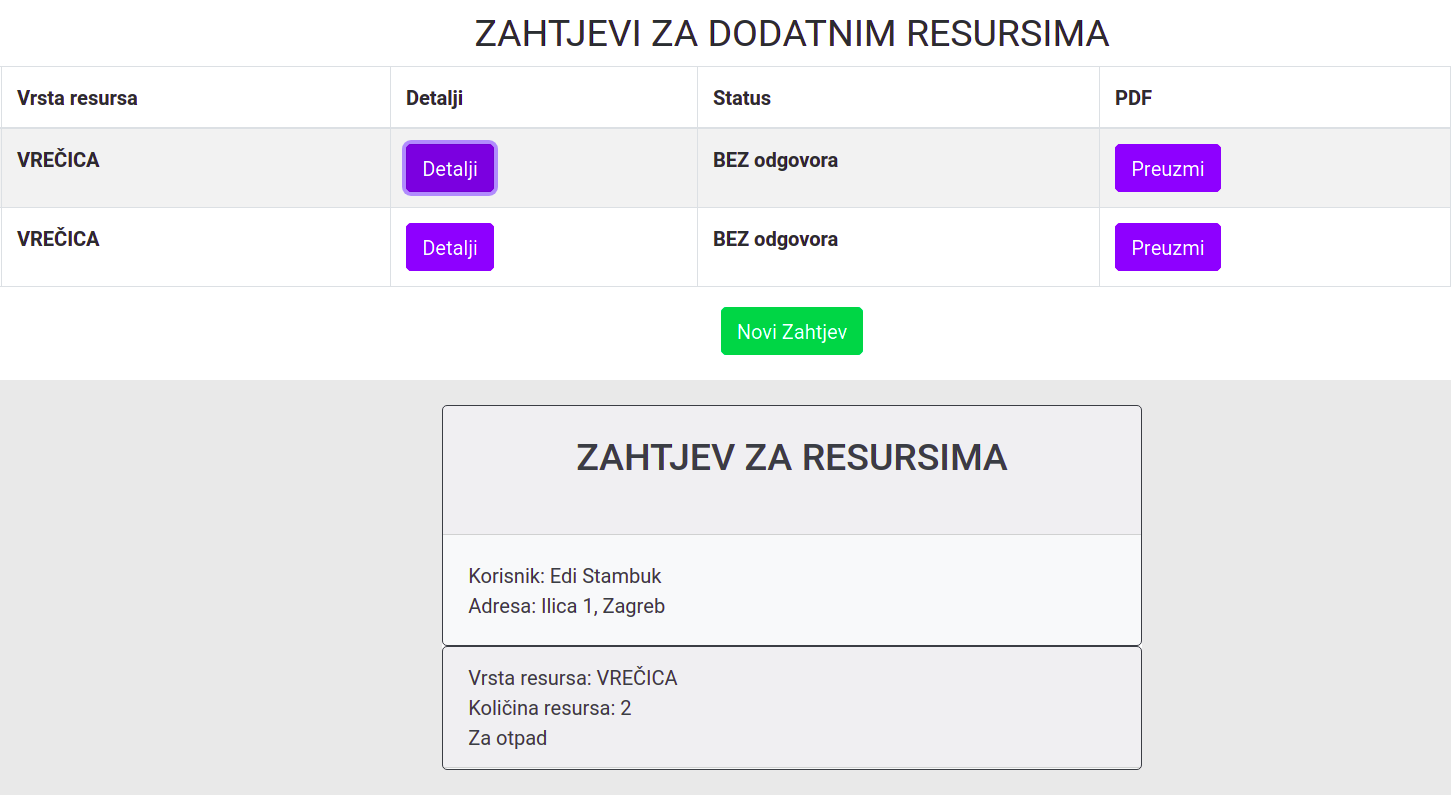
\includegraphics[scale=0.3]{slike/Zahtjev_resursi.png}
				\centering
				\caption{Zahtjev za resursima}
				\label{fig:Zahtjev_resursi}
			\end{figure}
			
			\text{}\\\\
			\text{}\\\\
		
			\textbf{Ispitni slučaj 4: Pretraga odgovarajućeg odlagališta za pojedini proizvod}
			\text{}\\\\
			
			\textbf{Ulaz:}
			
			\begin{packed_enum}
				\item{Otvaranje stranice za prikaz odgovarajućeg odlagališta za pojedini proizvod}
				\item{Upisivanje i odabir proizvoda za odlaganje}
				\item{Pritisak na gumb odlaganje}
			\end{packed_enum}
			
			\textbf{Očekivani rezultat:}
			
			\begin{packed_enum}
				\item{Pojavljivanje odgovarajućeg tipa odlagališta}
			\end{packed_enum}
			
			\textbf{Rezultat:} Korisnik je uspješno dobio odgovarajući tip odlagališta. Aplikacija je prošla test
			
			\begin{figure}[H]
				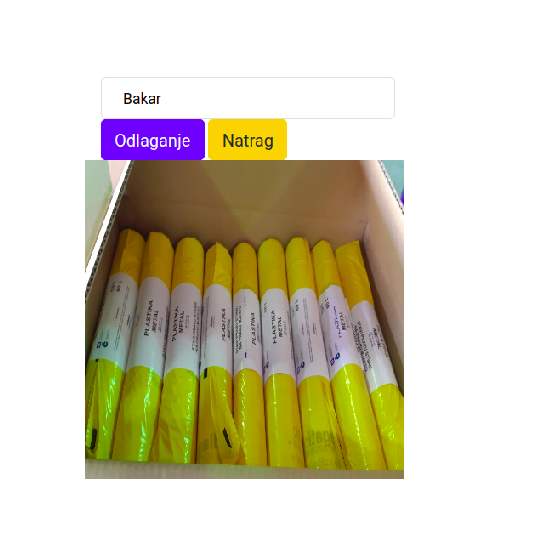
\includegraphics[scale=0.6]{slike/Tip_odlagalista.png}
				\centering
				\caption{Pronalazak odgovarajućeg tipa odlagališta}
				\label{fig:Tip_odlagalista}
			\end{figure}
			
			
			\eject 
		
		
			\section{Dijagram razmještaja}
		
		%			\textbf{\textit{dio 2. revizije}}\\
		
		
		Dijagrami razmještaja prikazuju računalne resurse koji su neophodni za ispravno funkcioniranje sustava i njihove međusobne odnose: stvarne uređaje (poslužitelje, radne stanice, korisnička računala, itd.), komponente programske podrške koje se na njima izvršavaju i veze između
		prikazanih resursa. Na računalu poslužitelja nalaze se poslužitelj baze podataka i web poslužitelj. Korisnik preko web poslužitelja pristupa sadržaju web aplikacije. HTTP veza je zaslužna za interakciju između korisnika i poslužitelja, dok je cijeli sustav građen na arhitekturi "klijent-poslužitelj", koja je jedna od najprimjenjivanijih metoda današnjice.
		
		
		\begin{figure}[H]
			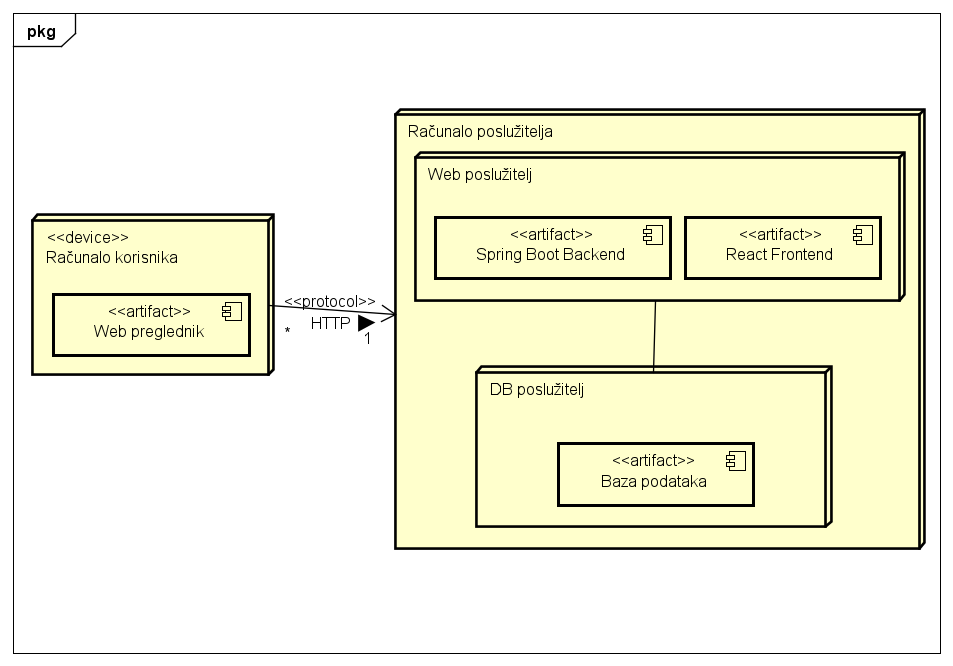
\includegraphics[width=\linewidth]{dijagrami/Deployment Diagram.png}
			\centering
			\caption{Dijagram razmještaja}
			\label{fig:dijagram_razmještaja}
		\end{figure}
	\newpage
		
		
		\section{Upute za puštanje u pogon}
		
%			\textbf{\textit{dio 2. revizije}}\\
%		
%			 \textit{U ovom poglavlju potrebno je dati upute za puštanje u pogon (engl. deployment) ostvarene aplikacije. Na primjer, za web aplikacije, opisati postupak kojim se od izvornog kôda dolazi do potpuno postavljene baze podataka i poslužitelja koji odgovara na upite korisnika. Za mobilnu aplikaciju, postupak kojim se aplikacija izgradi, te postavi na neku od trgovina. Za stolnu (engl. desktop) aplikaciju, postupak kojim se aplikacija instalira na računalo. Ukoliko mobilne i stolne aplikacije komuniciraju s poslužiteljem i/ili bazom podataka, opisati i postupak njihovog postavljanja. Pri izradi uputa preporučuje se \textbf{naglasiti korake instalacije uporabom natuknica} te koristiti što je više moguće \textbf{slike ekrana} (engl. screenshots) kako bi upute bile jasne i jednostavne za slijediti.}
%			
%			
%			 \textit{Dovršenu aplikaciju potrebno je pokrenuti na javno dostupnom poslužitelju. Studentima se preporuča korištenje neke od sljedećih besplatnih usluga: \href{https://aws.amazon.com/}{Amazon AWS}, \href{https://azure.microsoft.com/en-us/}{Microsoft Azure} ili \href{https://www.heroku.com/}{Heroku}. Mobilne aplikacije trebaju biti objavljene na F-Droid, Google Play ili Amazon App trgovini.}
			
			Aplikacija je javno dostupna na adresi \url{https://ezwaste.herokuapp.com/}
			
			
			 \subsection{Priprema baze podataka}
				\begin{enumerate}
					\item Na računalo instalirati neki od sustava za upravljanje bazom podataka (SUBP), u primjeru ćemo koristiti PostgreSQL. PostgreSQL SUPB se može preuzeti sa stranice \url{https://www.postgresql.org/}.
					\item Nakon preuzimanja, pokrenuti instalaciju i pri instalacija odabrati password koji će se koristiti za spajanje na 
					baze podataka koje se poslužuju na lokalnom poslužitelju. (username će biti 'postgres', password koji ćemo odabrati za primjer je 'admin'). Također tijekom instalacije potrebno je označiti opciju 'pgAdmin4'. To je program koji ima grafičko sučelje kroz koje korisnici mogu stvarati baze podataka i raditi upite nad njima.
					\item U sučelju programa pgAdmin4, pod rubrikom Servers odabrati PostgreSQL (11/12/...) server i povezati se s username i password koji ste prethodno odabrali.
					\item Desni klik na 'Databases', zatim 'Create', pa 'Database...'. U sljedećem prozoru unesite neko ime baze podataka (npr. 'ezwaste' za našu aplikaciju).
					\item Desni klik na ime baze podataka koju ste napravili, zatim 'Query tool...'. Sada će vam biti otvoren prozor u kojem možete izvršavati upite nad bazom 
					podataka. U prozor kopirajte sadržaj datoteke 'ezwaste\_create\_tables.sql' i pokrenite naredbe s tipkom F5.
					\item Ako želite osim tablica, u bazu unijeti i neke podatke za te tablice, onda napravite isti postupak kao u koraku prije, ali za datoteku 'insert\_data.sql'.
					\item U ovom trenutku će vam sve tablice biti stvorene u bazi podataka i možete krenuti na povezivanje aplikacije na lokalnu bazu podataka.
					\item U datoteci application.properties nalazi se sva konfiguracija koju backend aplikacija treba za povezivanje na bazu podataka.
					\item Ako ste pratili sve korake, ovako treba izgledati konfiguracija koju upisujete u application.properties datoteku:\\
					spring.datasource.url = jdbc:postgresql://localhost:5432/ezwaste\\
					spring.datasource.username = postgres \\
					spring.datasource.password = admin \\
					spring.jpa.hibernate.ddl-auto = none \\
					
				\end{enumerate}
			
				\subsection{Pokretanje backend aplikacije}
				\begin{enumerate}
					\item Za pokretanje backend aplikacije potrebno je otvoriti /izvorniKod/backend direktorij. U tom direktoriju se nalazi direktorij 'upravljanje-kucnim-otpadom',
					to je root direktorij našeg maven projekta kojeg otvorite u željenoj razvojnoj okolini (Intellij IDEA, Eclipse itd.)
					\item Spring boot aplikacija se pokreće tako da pokrenete (engl. run) main metodu koja se nalazi u 'UpravljanjeKucnimOtpadomApplication' klasi. 
					
				\end{enumerate}
			
				\subsection{Pokretanje frontend aplikacije}
				\begin{enumerate}
					\item Za pokretanje frontend aplikacije potrebno je imati instaliran Node.js\\
					 (\url{https://nodejs.org/en/}) te npm (dolazi uz Node.js).
					 \item Potrebno je "reći" frontend aplikaciji na kojoj se adresi nalazi API kojeg koristi. Otvoriti src/store/BaseUrl i provjeriti konstantu 'POCETNA\_ADRESA', ako nije, postaviti ju na 'localhost:8080'.
					\item Aplikacije se pokreće tako da se pozicionirate u root direktorij projekta. /izvorniKod/frontend/upravljanje\_kucnim\_otpadom te u komandnoj
					liniji izvršite naredbe : \\
					-npm install \\
					-npm start
			
				\end{enumerate}
			
			
			\eject 